\documentclass[a4paper,12pt,abstracton]{scrartcl}
\usepackage[utf8]{inputenc}
\usepackage{float}
\usepackage{amsmath}
\usepackage{amssymb}
\usepackage{pifont}% http://ctan.org/pkg/pifont
\usepackage[font=small,labelfont=bf]{caption}
\usepackage{graphicx}
\usepackage{dirtytalk}
\usepackage{multicol}
\usepackage{booktabs}
\usepackage{colortbl}
\usepackage{appendix}
\usepackage{nomencl}
\usepackage{lmodern}
\usepackage[nottoc]{tocbibind}
\usepackage{xcolor}
%\graphicspath{images/}
\usepackage[margin = 3cm]{geometry}
\usepackage{ragged2e} % good alignment
\usepackage{hyperref}
\usepackage{siunitx} % Provides the \SI{}{} and \si{} command for typesetting SI units
\hypersetup{colorlinks=true,
    linkcolor=blue,
    filecolor=magenta,      
    urlcolor=cyan, 
    citecolor=gray}

%\DeclareGraphicsExtensions{.png,.pdf} % low-res (work in progress)
%\DeclareGraphicsExtensions{.pdf,.png}  % high-res (final draft)
%\setlength\parindent{0pt} % Removes all indentation from paragraphs
%\bibliographystyle{unstr}
\setlength\parindent{0pt}
\setlength{\parskip}{0.3em}
\newcommand{\xmark}{\ding{55}}

\renewcommand{\nomname}{List of Symbols}
\renewcommand{\nompreamble}{The following list explains the symbols used within the body of the report.}

\begin{document}

\begin{figure}[H]
    \centering
    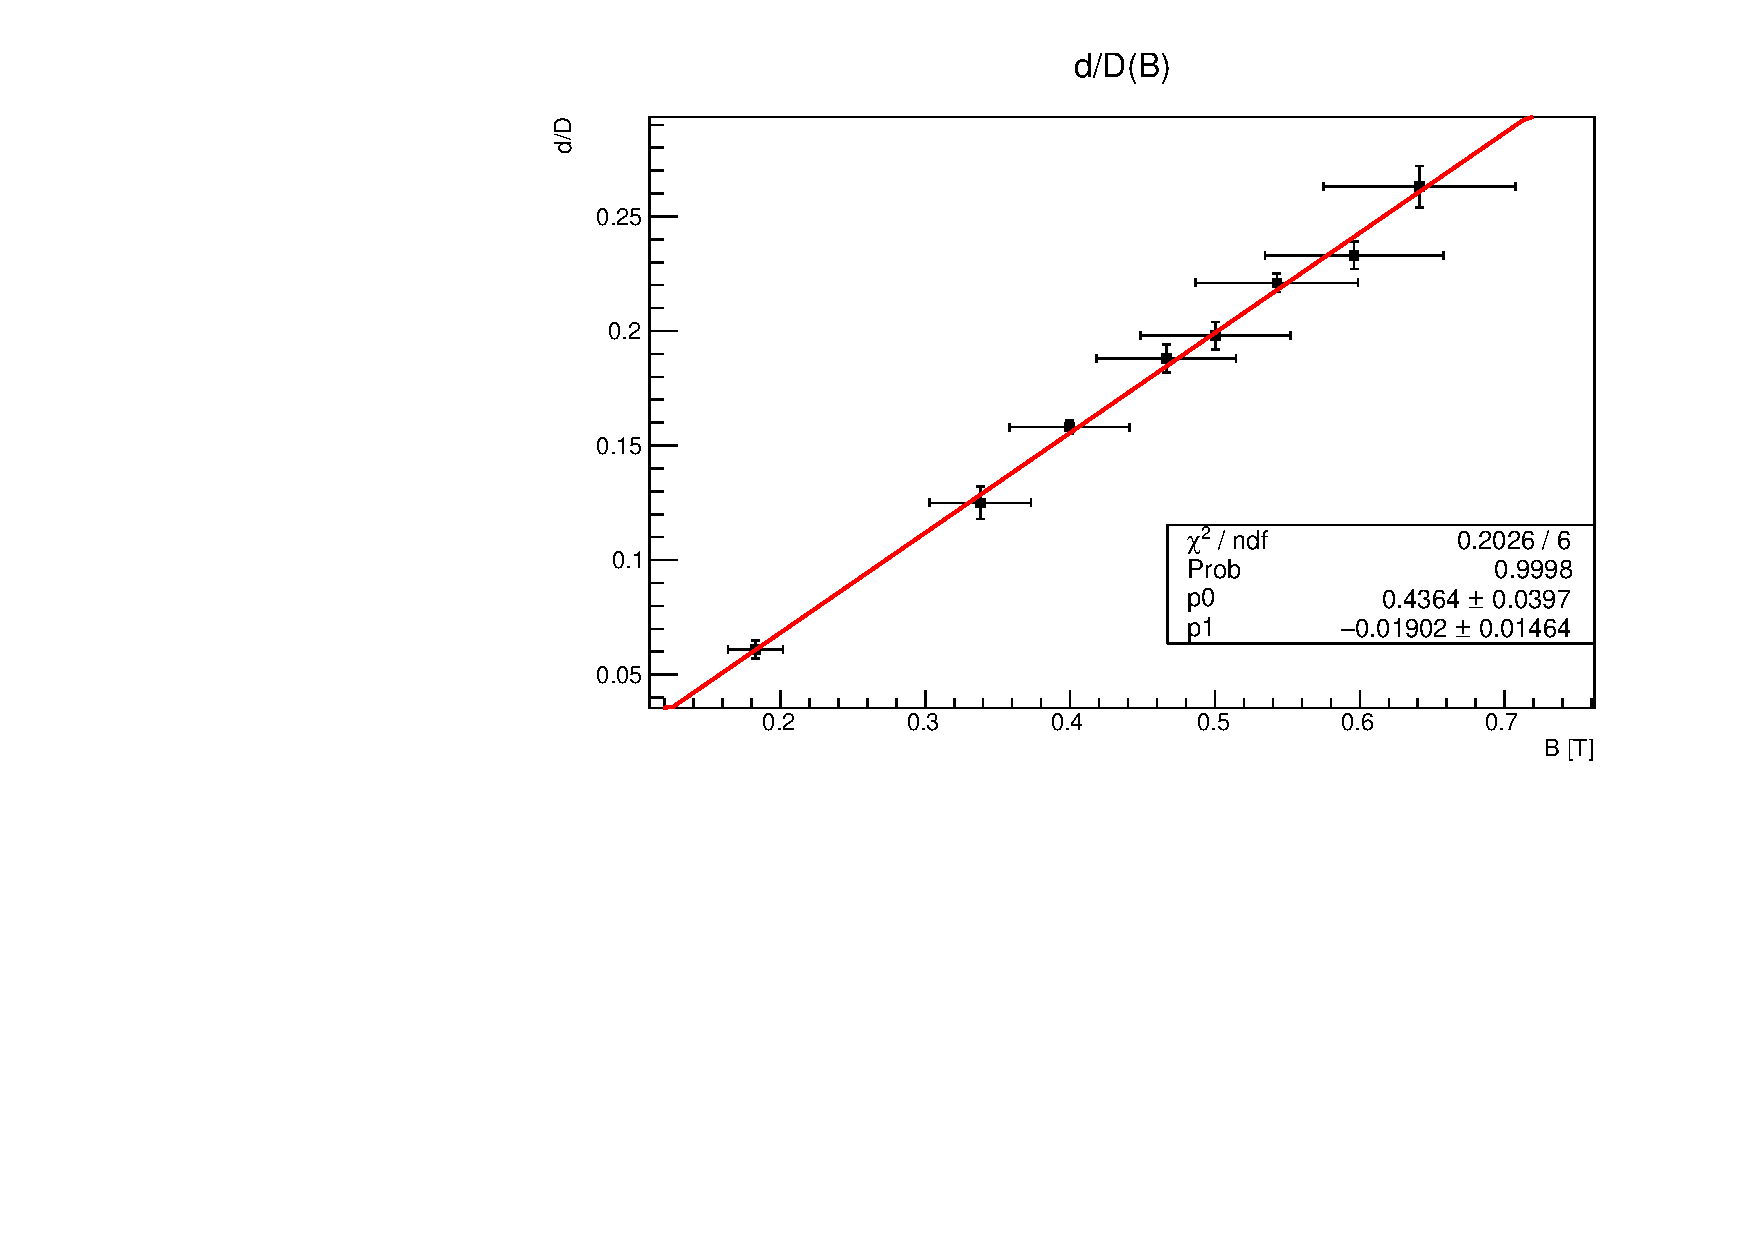
\includegraphics[scale=0.6]{plots/znt.pdf}
    \caption{}
    \label{fig:znt}
\end{figure}

\begin{figure}[H]
    \centering
    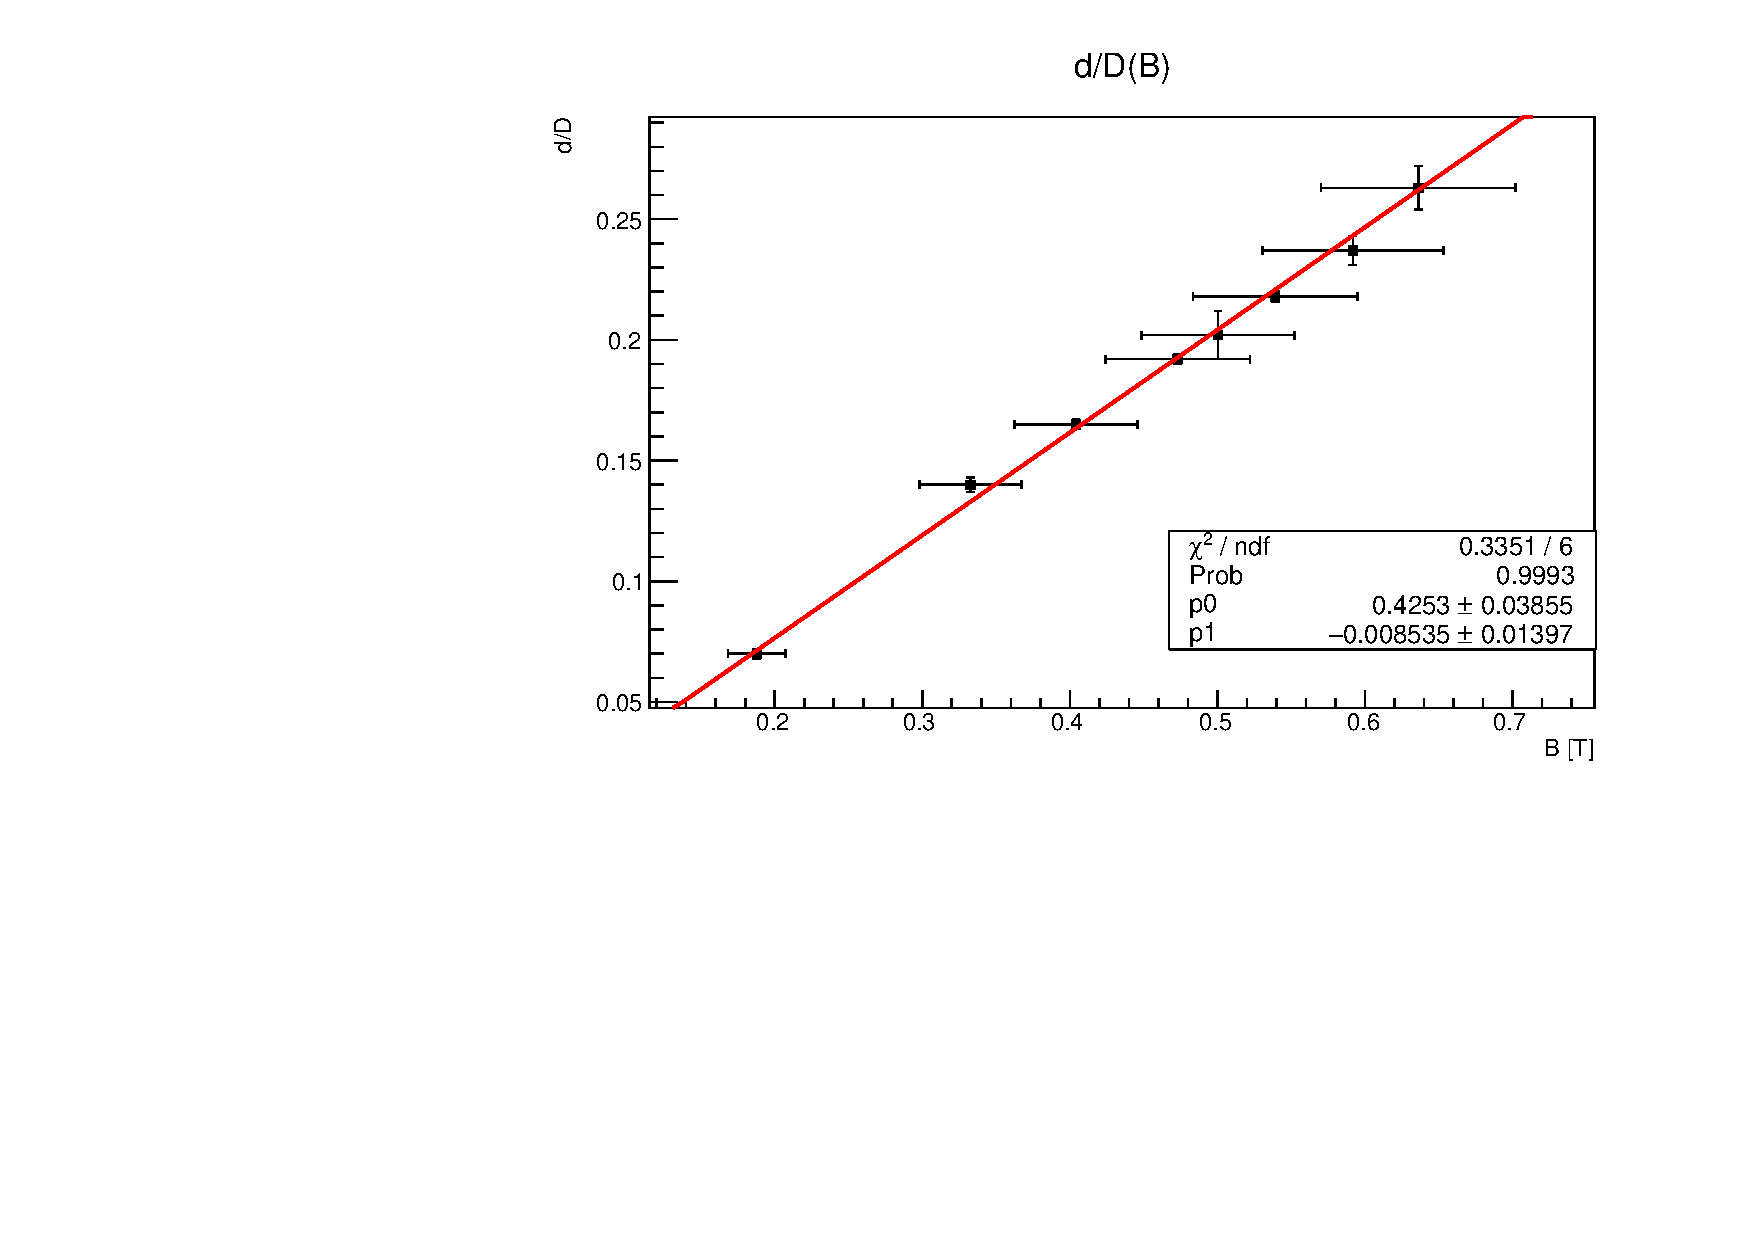
\includegraphics[scale=0.6]{plots/znl.pdf}
    \caption{}
    \label{fig:znl}
\end{figure}

\begin{figure}[H]
    \centering
    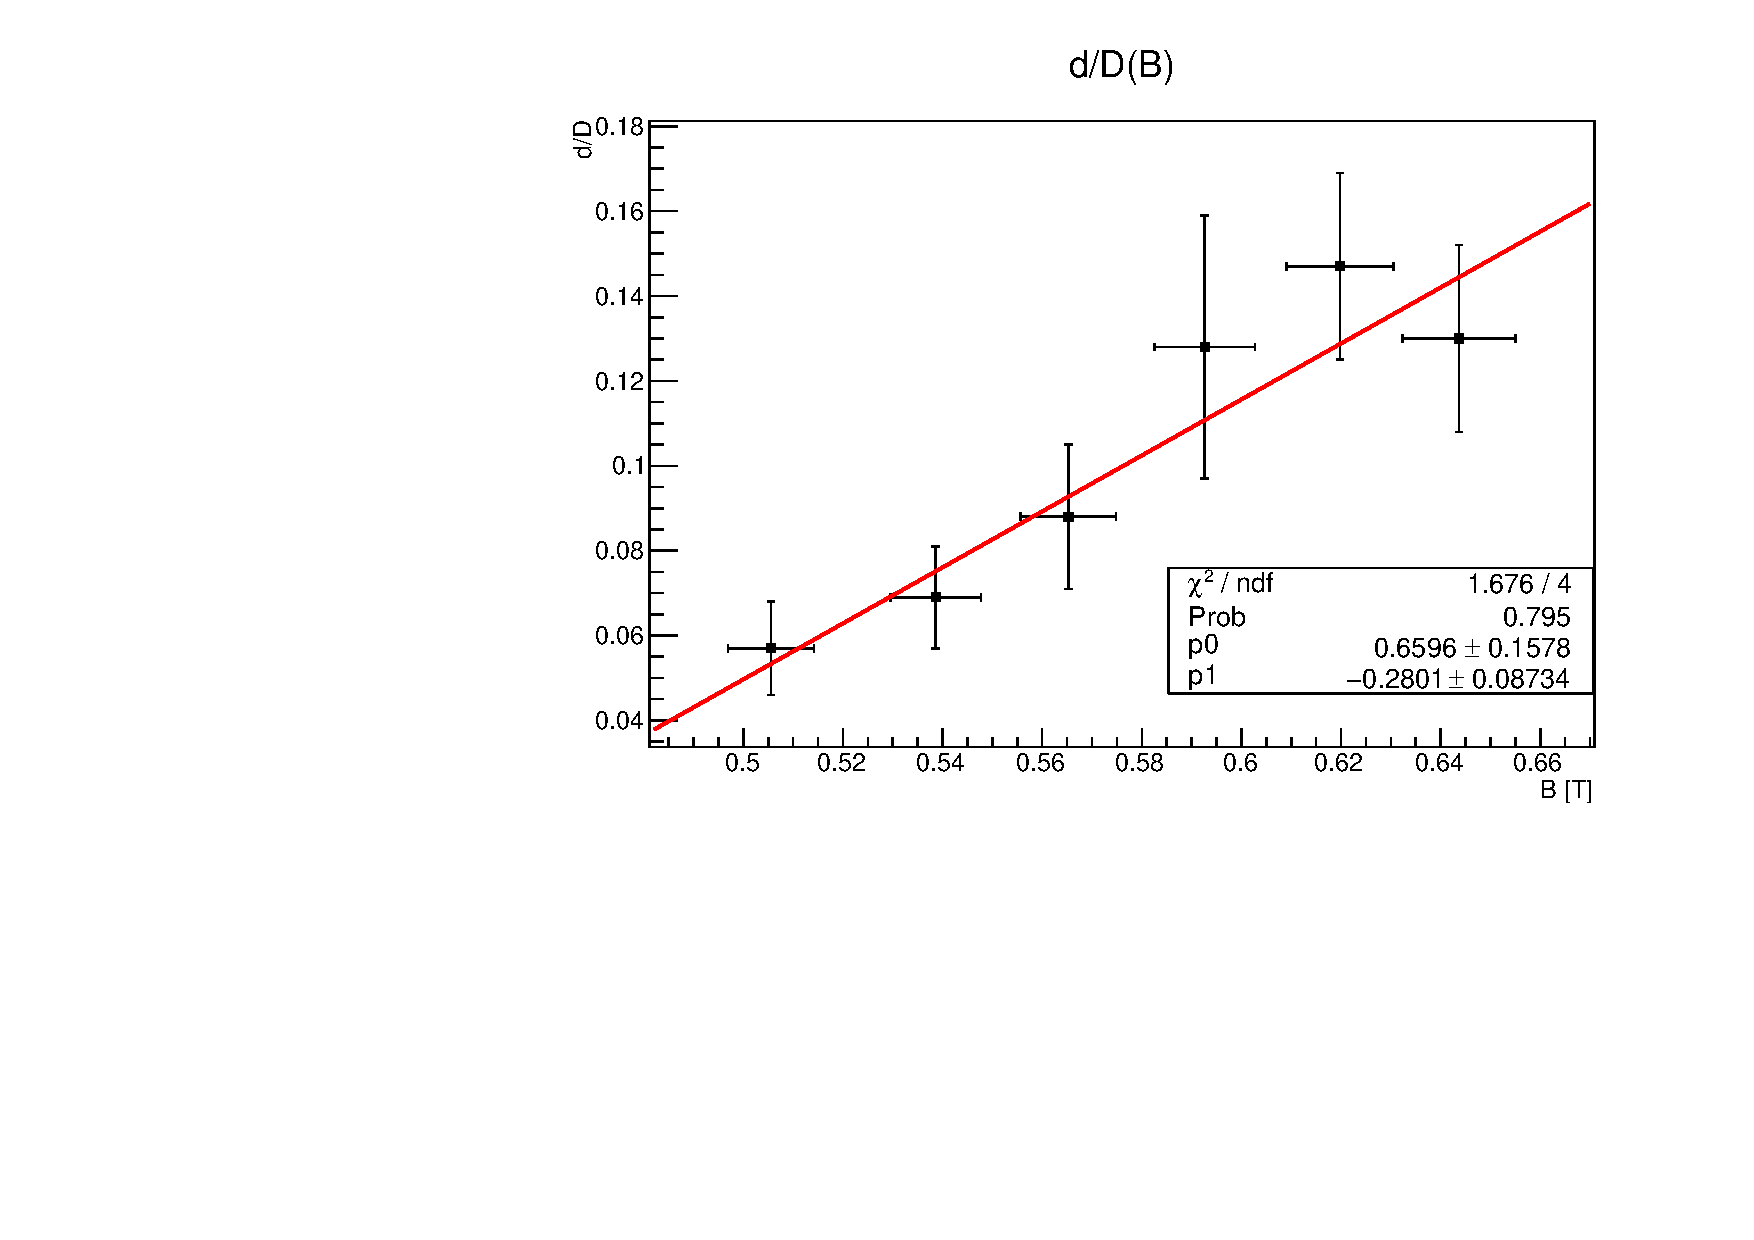
\includegraphics[scale=0.6]{plots/zal.pdf}
    \caption{}
    \label{fig:zal}
\end{figure}

\begin{figure}[H]
    \centering
    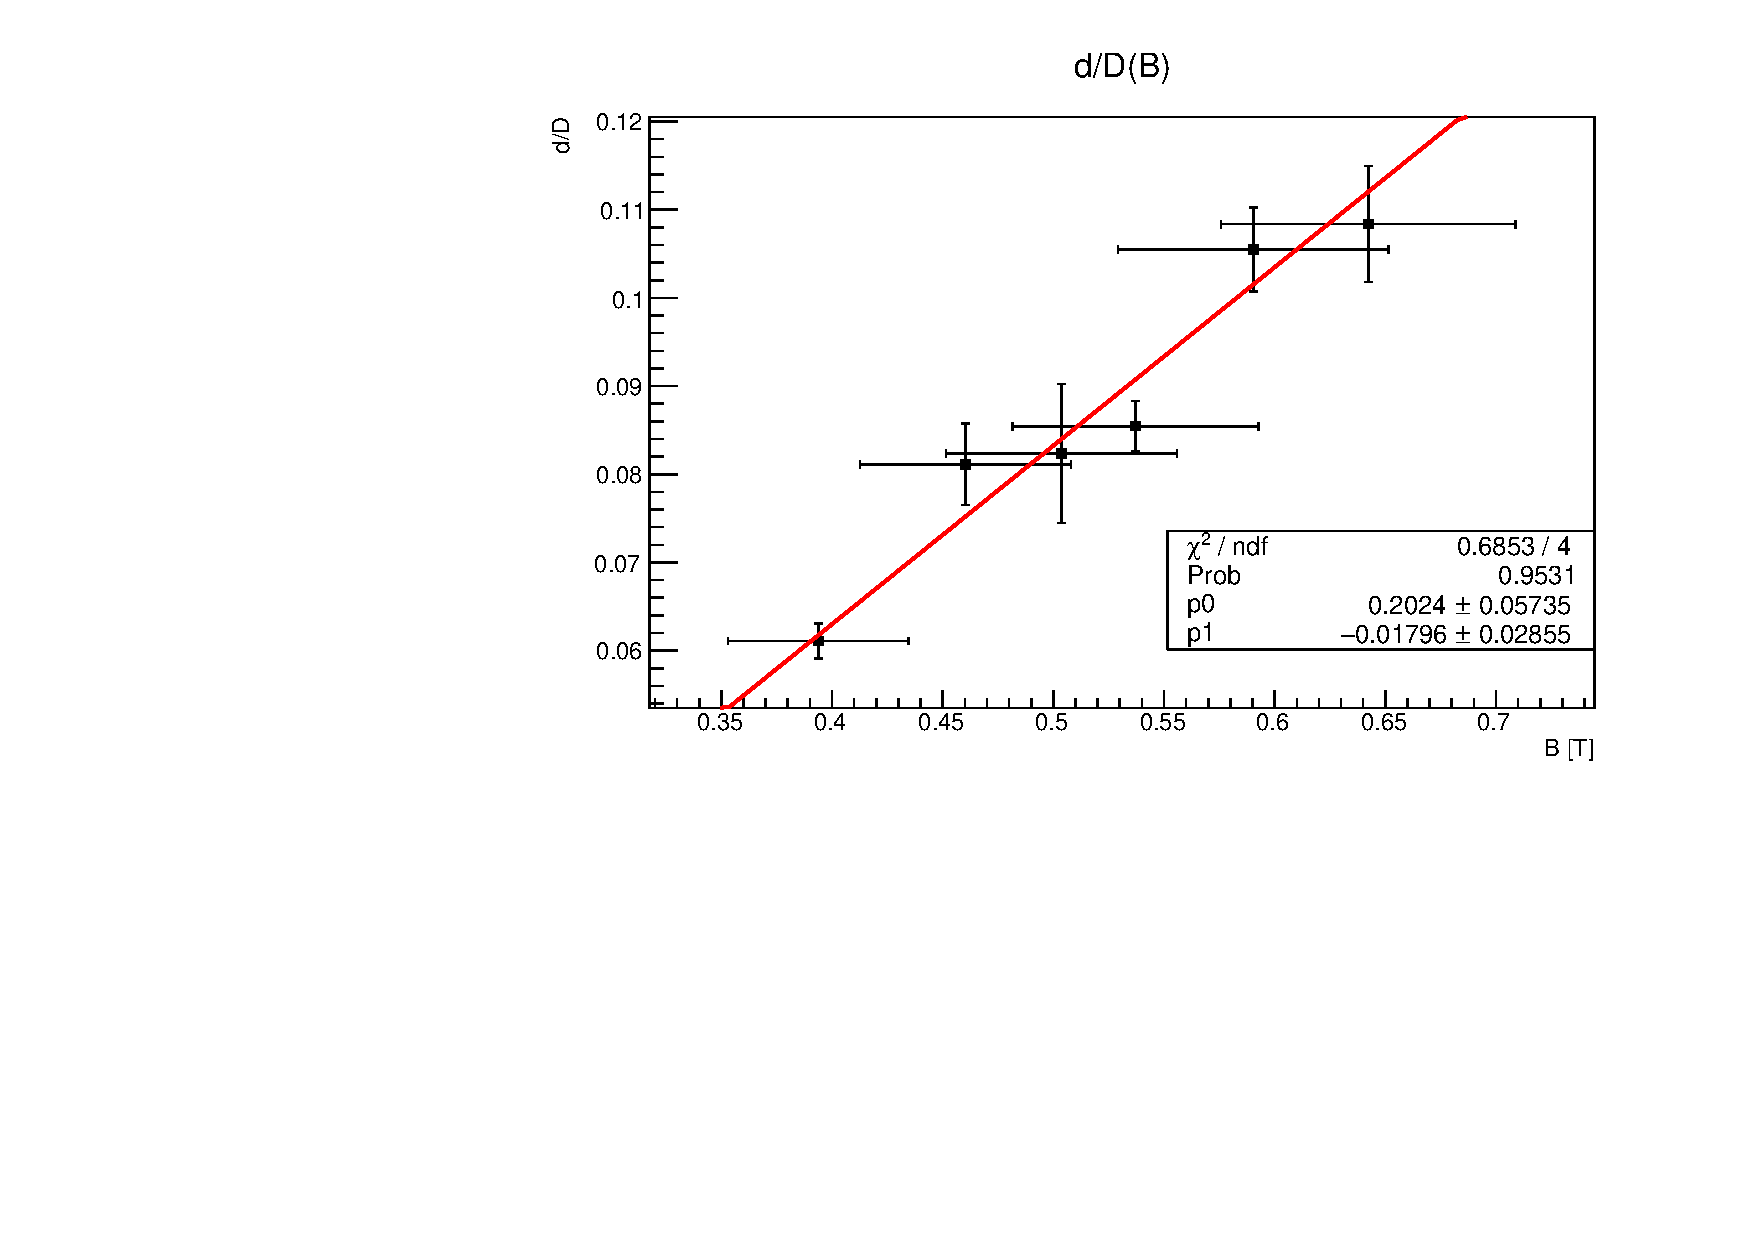
\includegraphics[scale=0.6]{plots/zatbs.pdf}
    \caption{}
    \label{fig:zat}
\end{figure}

\end{document}